
ElecSIM has been designed for ease of use to enable non-experts to rapidly test different policies and the outcome of various scenarios such as demand growth. The user is able to input exogenous variables such as fuel cost, carbon taxes, power plants, power plant costs, electricity demand and availability factors. This allows for the initialisation of different countries and scenarios to be tested.


\subsection{High-Level Overview}

A schematic of ElecSIM is displayed in Figure \ref{fig:system_overview}. We have provided data sources to calibrate the model, for instance, historical fuel prices, historical plant availability, wind and solar capacity, power plant costs, historical costs, historical efficiency, company finances and historical carbon price. Unless otherwise stated, these data have been calibrated to the UK or Europe.

The configuration file give the ability to the user to rapidly change scenarios, and points to the various previously mentioned data sources. This data is then used to calibrate the GenCos and demand agent. GenCos then invest in power plants based on the highest positive net present value (NPV). Bids are made for each power plant based on the power plants short run marginal cost. A power exchange operator matches these bids with demand in merit order. 

This is then repeated for each year of the simulation.


\begin{figure}[h]
	\begin{center}
		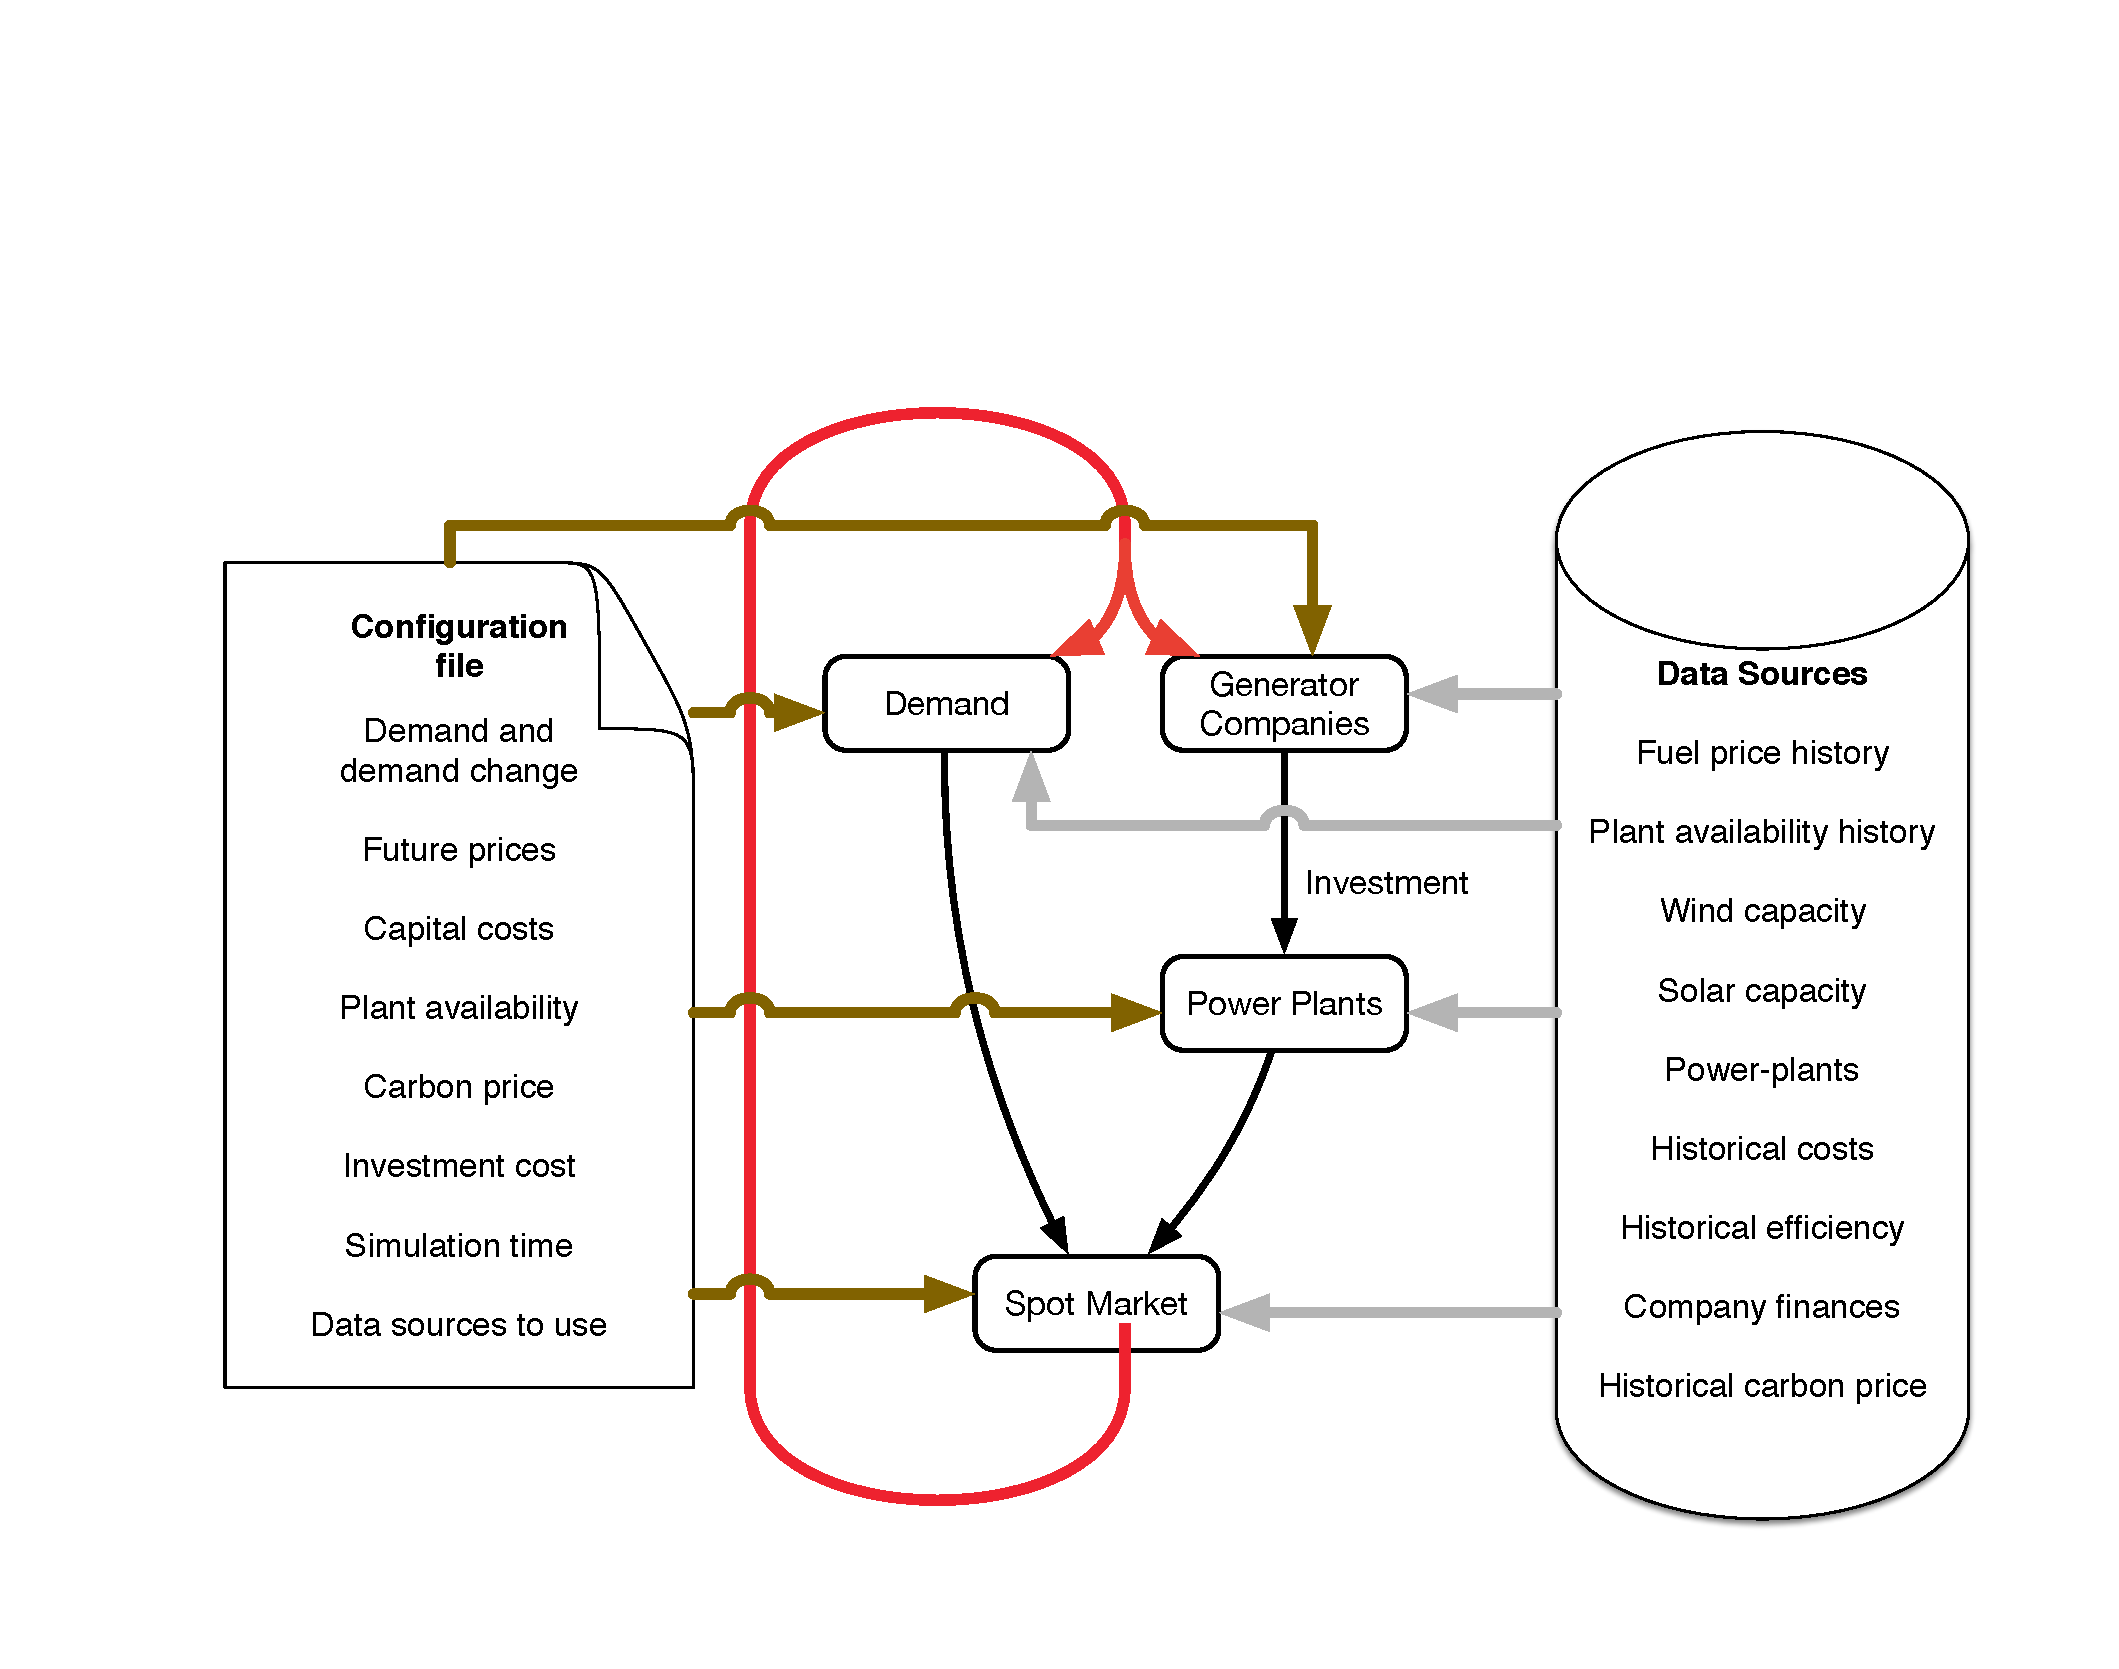
\includegraphics[width=0.5\textwidth]{figures/System_overview.pdf}
		\caption{ElecSIM simulation overview}
		\label{fig:system_overview}
	\end{center}
\end{figure}

\subsection{Detailed Overview}

ElecSIM is made up of two different agent types, GenCos (Generation Companies) and a Demand agent. GenCos can be initialised by the user. For example, to a desired country, or a toy-example. Each of the GenCos are initialised with their respective power plants. GenCos are given a randomized discount rate, which can be set by the user, around a mean of 10\% for nuclear power plants \cite{Paper2012} and 5.9\% for all other generators \cite{KPMG2017}.

\subsubsection{Data Initialisation}ElecSIM's power generation costs is initialised using the UK government Department for Business, Energy and Industrial Strategy (BEIS) power plant generation report \cite{Department2016}. This contains information such as capital costs and operation and maintenance costs, including details such as insurance and connection costs. Where there are power plants of a size not included in this report, the parameters are linearly interpolated. Where the capacity of a power plant is larger or smaller than the data points in the report, the parameters are extrapolated by using the last known data point.

For historical power plants, we used historical costs of Levelised Cost of Energy (LCOE) \cite{Dale2013}. Each parameter was scaled linearly from the modern LCOE calculated from the BEIS report, to attain the relevant historical LCOE. This was achieved by using linear optimisation, and therefore each parameter can be changed based on an individual user's country and dataset by modifying these constraints. As well as historical LCOE, historical plant efficiency was taken into account for gas and coal power plants \cite{EIA2013}.

When initialised, the variable operation and maintenance costs are selected from a uniform distribution, with the ability for the user to set maximum and minimum percentage increase from the BEIS report. A uniform distribution was chosen to capture the large deviations that can occur in variation of variable operation and maintenance. By doing this, the variance in costs between individual power plants for processes such as preventative and corrective maintenance, labour costs and skill, health and safety and chance.  

As per \cite{Chappin2017}, we created a load duration curve of the electricity demand for one year with 20 segments. 20 segments enabled us to capture the varying demand of electricity throughout a year to a high enough degree of accuracy, but also reduce computational complexity. To model the Intermittency of wind and solar power we allow them to contribute only a certain percentage of total capacity for each load segment based on empirical wind and solar capacity factors, relating demand to average capacity \cite{Pfenninger2016, Staffell2016, Chappin2017}. The requirement of storage to provide constant electricity from intermittent resources is an important issue. However, due to ElecSIM taking yearly time steps, we are unable to model short term variability in electricity demand. We also, do not model long-term storage due to its currently limited liability. 

However, we do not model curtailment of renewables, or storage capabilities. 

Whilst fuel price is controlled by the user, there is inherent volatility in fuel price in a single year. To take into account this variability, an ARIMA model was fit to historical gas and coal price data \cite{coalprices,gasprices}. The standard deviation of the residuals was used to model the price of fuel that a generation company will buy fuel at in a given year. This takes into account differences in hedging strategies and chance between generation companies.

Outages are modelled by using availability data of gas, coal, photovoltaic, offshore and onshore power generators \cite{Ltd2016, Hunt2015, carroll-j}. Plants bid a reduced percentage of their nameplate capacity based on their respective availability. Historical availabilities are modelled for older gas, coal and hydro power plants \cite{AlbertaSystemElectricOperator2016}.

With historical power plants which have been refurbished, we sample their initialisation randomly between 15 years prior to initialisation year and the initialisation year.

Power plants are taken out of service if they have not sold any electricity in the past 7 years. We decided upon this due to the fact that power generators have high, sunk capital costs, which often have high demolition costs. We assume, therefore, that generator companies are willing to wait circa $\frac{1}{4}$ of their lives to see if a pay-out occurs due to the breakdown of competing power plants, increasing demand, or governmental support in the form of a carbon tax increase or reduction.


\subsubsection{Spot Market}

The buying and selling of electricity is modelled as a spot market, where each year, electricity is bought and sold in merit order. GenCos place bids for each of their plants at their respective short run marginal cost. We assume that generator companies do not have market power, however we set the lost load to be \textsterling6000 to encourage investment as per the recommendations of the UK government \cite{DECC2013}.

\subsubsection{Investment}

Investments are made on a yearly basis and are made purely on net present value calculations. The order in which GenCos invest in each simulated year is randomised as to not give certain generation companies an advantage.

Agents have imperfect information, and therefore fuel and carbon prices are predicted using linear regression, with a training period sampled uniformly from 3 to 7 years back. This allows us to model heterogeneity of GenCos. Demand is modelled through the use of an exponential function, so that compounded growth can be modelled. However, if a reasonable fit for the previous data is not found, a linear regression is used.

GenCos only bid if they have 25\% of the upfront capital costs, with the rest of the capital provided through equity and debt. The cost of equity and debt is modelled as a weighted average cost of capital (WACC), with values of 5.9\% for non-nuclear power plants, and 10\% for nuclear power plants \cite{KPMG2017, Paper2012}. The WACC is used as the discount rate for net present value calculations \cite{KincheloeStephenC1990TWAC}. Each GenCo is initialised with a slightly different discount rate based on a uniform distribution, with a $\pm$3\% standard deviation. This allows us to model the variability in discount rates that GenCos may have, based on different factors such as preference, confidence in the future and readiness for investors and lenders to supply capital.

The sale price of electricity in the future reference year is predicted by each generation company simulating the same merit-order market algorithm that is used for the spot market. They simulate the bids that they expect each of the power plants that are in operation to make, and use the demand predicted to match supply with demand. They then assess whether their investment option is likely to make a profit, ie. with a positive net present value. The power plant with the highest net present value is then invested in. 





\begin{itemize}
	\item Model can be modified through a single python scenario file which includes exogenous variables such as number of generation companies, power plants, power plant costs, tax and fuel prices, and demand.
	\item Architectural framework:
	\begin{itemize}
		\item Agents are generation companies.
		\item Generation companies initialized from government data. And randomized discount rate around a mean of 10\% for nuclear power plants and 5.9\% for other types of generators.
		\item Costs of power plants taken from empirical data. 
		\item Historical LCOE costs taken from data, with individual costs such as fixed operation and maintenance, construction and pre-development costs scaled linearly to match LCOE value. (This can be changed by user by specifying linear optimisation constraints).
		\item Historical Gas turbine and Coal plant efficiency taken from epa data.
		\item Variable operation and maintenance costs are stochastic to take into account differences in design types, preventative and corrective maintenance, labour costs and skill, asset and site management, health and safety and chance.
		\item Electricity demand taken from historical data and split up into 19 load segments.
		\item CO2 prices, fuel Prices, demand growth are exogenous
		\item Fuel is bought by power producers each year at different prices, related to the standard deviation from historical data. This simulates different hedging strategies, luck and timing of fuel purchasing.
		\item Outages are modelled by assuming a 93\% outage rate for fuel plants \cite{Ltd2016} and 97\% outage for renewables. \cite{carroll-j}
		\item Generation companies bid their short run marginal costs.
		\item Investments made on highest Net Present Value results. CO2 price, fuel price and demand are predicted 7 years ahead using linear regression. 
		\item Estimated sale of electricity price calculated by simulating a market 7 years into the future with expected power plants that are running and have been taken out of service.
		\item Investors will only invest if they have 25\% of the total upfront costs. (the rest taken on by debt and equity as assumed by WACC value.)
		\item Intermittent power generators can only submit a certain percentage of their total capacity for each load segment. This percentage is matched with empirical data.
		\item Bids accepted by a centralised power exchange based on merit order. Generation companies bid their short run marginal cost.
	\end{itemize}
	\item Assumptions: 
	\begin{itemize}
		\item Yearly time step
		\item Renewables contribute to load curve of each demand segment matched with empirical data of typical wind and solar availability at each demand segment
		\item Different discount rates per user (randomized)
		\item Country initialized with full amount of power plants and generation companies in country and total demand data considered
		\item No curtailment of renewables
		\item Imperfect foresight - Prediction required for demand, co2 price, fuel cost, other investments.
		\item Power plant construction and pre-development periods and costs modelled from UK Government BEIS data
		\item Investments based on highest NPV using a single year 7 (can be changed in scenario file) time steps into the future to predict all years of power plant.
		\item Agents predict next year's fuel, carbon and demand using linear regression and randomized look back period (between 3 and 6.)
		\item Plants are dismantled after their lifetime, and only enter operation after pre-development/construction.
		\item Legacy power plants are reinitialized to random starting year to account for refurbishment.
		\end{itemize}
\end{itemize}